\documentclass[11pt]{article}
\usepackage{graphicx}
\usepackage[mathletters]{ucs}

\usepackage{float}
\usepackage[utf8x]{inputenc}
\usepackage[polish]{babel}
\usepackage[T1]{fontenc}
\usepackage{titlesec}
\usepackage{array}
\usepackage{multirow}
\setcounter{secnumdepth}{4}
\titleformat{\paragraph}
{\normalfont\normalsize\bfseries}{\theparagraph}{1em}{}
\titlespacing*{\paragraph}
{0pt}{3.25ex plus 1ex minus .2ex}{1.5ex plus .2ex}
\graphicspath{ {images/} }
\newcolumntype{L}[1]{>{\raggedright\let\newline\\\arraybackslash\hspace{0pt}}m{#1}}
\newcolumntype{C}[1]{>{\centering\let\newline\\\arraybackslash\hspace{0pt}}m{#1}}
\newcolumntype{R}[1]{>{\raggedleft\let\newline\\\arraybackslash\hspace{0pt}}m{#1}}
\begin{document}
\title{Struktury danych i złożoność obliczeniowa}
\author{Łukasz Wdowiak}
\begin{titlepage}
    \begin{center}


        \vspace*{-3cm}

        
\includegraphics[width=14cm]{images/image.png}

        \vspace*{2cm}
        \huge
        \textbf{Badanie efektywności algorytmów grafowych w zależności od rozmiaru instancji oraz sposobu
            reprezentacji grafu w pamięci komputera.}

        \vspace{0.5cm}


        \vspace{1.5cm}

        \textbf{Łukasz Wdowiak}

        \vspace{2cm}

        \vfill
        Prowadzący: dr inż. Dariusz Banasiak \\
        Grupa: K03-37h, Pon 15:15-16:55 TP \\
        \vspace{2cm}
        Wydział Informatyki i Telekomunikacji \\
        Informatyka Techniczna \\
        IV semestr\\




    \end{center}
\end{titlepage}

\section{Wstęp teoretyczny}
Badanie efektywności algorytmów grafowych w zależności od rozmiaru instancji oraz sposobu reprezentacji grafu w pamięci komputera jest ważnym obszarem badań w dziedzinie informatyki i algorytmiki.
Algorytmy grafowe są używane do rozwiązywania różnorodnych problemów związanych z grafami, takich jak wyszukiwanie najkrótszej ścieżki czy minimalne drzewo rozpinające.

Efektywność algorytmów grafowych może być mierzona na różne sposoby, ale dwa kluczowe czynniki to rozmiar instancji oraz sposób reprezentacji grafu w pamięci komputera.
Rozmiar instancji odnosi się do liczby wierzchołków i gęstości grafu. Gęstością grafu nazywamy stosunek liczby krawędzi do liczby wierzchołków.
Im większy graf, tym więcej operacji trzeba wykonać, co może wpływać na czas wykonania algorytmu.

Sposób reprezentacji grafu w pamięci komputera również ma duże znaczenie dla efektywności algorytmów grafowych.
Istnieje wiele sposobów reprezentacji grafu, takich jak macierze incydencji czy listy sąsiedztwa.
Każda z tych reprezentacji ma swoje zalety i wady pod względem szybkości działania i zajmowanej pamięci.

Algorytmy najkrótszej ścieżki (Dijkstra, Bellman-Ford) oraz algorytmy minimalnego drzewa rozpinającego (Prim, Kruskal) są ważnymi narzędziami w teorii grafów.
Algorytm Dijkstry znajduje najkrótszą ścieżkę w grafie skierowanym, podczas gdy Bellman-Ford radzi sobie również z krawędziami o ujemnych wagach. Algorytmy Prima i Kruskala znajdują minimalne drzewo rozpinające w grafie nieskierowanym.
Efektywność tych algorytmów może zależeć od rozmiaru grafu, sposobu reprezentacji oraz problemu, który jest rozwiązywany.

\section{Reprezentacja grafu}
Reprezentacja grafu to sposób przedstawienia grafu w pamięci komputera, który umożliwia skuteczne przetwarzanie i wykonywanie operacji na grafie.
Istnieją różne metody reprezentacji grafu, z których dwie popularne to macierz incydencji oraz lista sąsiedztwa.
\subsection{Macierz incydencji}
Macierz incydencji to dwuwymiarowa tablica, w której wiersze reprezentują wierzchołki, a kolumny reprezentują krawędzie.
W komórce macierzy znajduje się liczba reprezentująca wagę krawędzi lub 0 w przypadku braku krawędzi między danym wierzchołkiem a krawędzią.
W przypadku grafów skierowanych krawędzie są reprezentowane przez liczby ujemne i dodatnie, które oznaczają odpowiednio kierunek krawędzi.
Ta reprezentacja jest skuteczna w przypadku grafów o małej gęstości, gdzie liczba krawędzi jest stosunkowo niewielka.
Złożoność pamięciowa tego algorytmu wynosi $\  O(V * E) $, gdzie V to liczba wierzchołków, a E to liczba krawędzi.
Macierz incydencji wymaga pamięci proporcjonalnej do iloczynu liczby wierzchołków i krawędzi.

\subsection{Lista sąsiedztwa}
Lista sąsiedztwa to struktura danych, w której każdemu wierzchołkowi przypisywana jest lista jego sąsiadów. Ta lista przechowuje informacje o wierzchołkach, do których istnieje krawędź, oraz opcjonalnie informacje o wagach krawędzi.
Ta reprezentacja jest szczególnie przydatna dla grafów o dużej gęstości, gdzie liczba krawędzi może być znaczna.
Złożoność pamięciowa tego algorytmu wynosi $\  O(V + E) $, gdzie V to liczba wierzchołków, a E to liczba krawędzi.
Lista sąsiedztwa wymaga pamięci proporcjonalnej do sumy liczby wierzchołków i krawędzi.

\section{Najkrótsza ścieżka}
Algorytmy najkrótszej ścieżki, takie jak Dijkstra i Bellman-Ford, są używane do znajdowania najkrótszych ścieżek w grafach skierowanych lub nieskierowanych.
Ich celem jest znalezienie ścieżki o najmniejszej sumie wag krawędzi pomiędzy dwoma wierzchołkami w grafie.
\subsection{Algorytm Dijkstry}
Algorytm Dijkstry działa w sposób iteracyjny, przechodząc przez wierzchołki grafu, zaczynając od wierzchołka źródłowego.
Przypisuje początkową wartość odległości do każdego wierzchołka jako nieskończoność, a następnie aktualizuje te wartości, porównując je z wagami krawędzi.
Algorytm wybiera wierzchołek o najmniejszej aktualnej odległości i relaksuje wszystkie krawędzie wychodzące z tego wierzchołka.
Proces ten kontynuuje się, aż wszystkie wierzchołki zostaną odwiedzone.
Algorytm posiada złożoność czasowa $\ O(V^2) $, gdzie V to liczba wierzchołków w grafie przy reprezentacji macierzowej. Z kolei przy reprezentacji listowej złożoność wynosi $\ O(V + E * log(V)) $.

\subsection{Algorytm Bellmana-Forda}
Algorytm Bellmana-Forda również działa w sposób iteracyjny, ale może radzić sobie z krawędziami o ujemnych wagach.
Algorytm rozpoczyna się od przypisania początkowych odległości dla wszystkich wierzchołków jako nieskończoność, a odległość do wierzchołka źródłowego jako 0.
Następnie relaksuje krawędzie iteracyjnie, sprawdzając, czy można skrócić odległość do danego wierzchołka, poprzez wykorzystanie innych wierzchołków.
Algorytm powtarza te kroki V-1 razy, gdzie V to liczba wierzchołków w grafie, aby upewnić się, że wszystkie najkrótsze ścieżki zostały znalezione.
Algorytm posiada złożoność czasowa $\ O(V * E) $, gdzie V to liczba wierzchołków w grafie, a E to liczba krawędzi.

\section{Minimalne drzewo rozpinające}
Algorytmy Prim i Kruskala są wykorzystywane do znajdowania minimalnego drzewa rozpinającego w grafach nieskierowanych, czyli drzewa, które łączą wszystkie wierzchołki grafu, minimalizując sumę wag krawędzi.
\subsection{Algorytm Prima}
Algorytm Prima rozpoczyna się od wybranego wierzchołka i stopniowo rozbudowuje minimalne drzewo rozpinające poprzez dołączanie kolejnych krawędzi o najmniejszej wadze.
Na każdym kroku wybierany jest wierzchołek, który jest najbliżej istniejącego drzewa, i dodawana jest do niego najkrótsza krawędź.
Proces ten kontynuuje się, aż wszystkie wierzchołki zostaną odwiedzone i drzewo zostanie ukończone.
Algorytm ten posiada złożoność czasową $\ O(V^2) $, gdzie V to liczba wierzchołków w grafie przy reprezentacji macierzowej. Z kolei przy reprezentacji listowej złożoność wynosi $\ O(V + E * log(V)) $.
\subsection{Algorytm Kruskala}
Algorytm Kruskala działa na podobnej zasadzie, ale zamiast rozszerzać minimalne drzewo rozpinające od jednego wierzchołka, sortuje wszystkie krawędzie w kolejności rosnącej wag i stopniowo dodaje je do drzewa.
Krawędzie są dodawane do drzewa, jeśli nie tworzą cyklu z już dodanymi krawędziami.
Proces ten kontynuuje się, aż wszystkie wierzchołki zostaną połączone w jedno drzewo.
Algorytm ten posiada złożoność czasową $\ O(E * log(V)) $.


\section{Plan projektu}
\subsection{Zarys projektu}
\begin{itemize}

    \item Program napisansy został w języku C++, bez wykorzystywania biblioteki STL.
          Projekt implementuje cztery algorytmy grafowe: Dijkstry, Bellmana-Forda, Prima i Kruskala.

    \item Zaimplementowane algorytmy są testowane na grafach o różnych rozmiarach i gęstościach. Waga krawędzi jest losowana z przedziału od 1 do 10.

    \item Wszystkie struktury danych są alokowane dynamicznie.

    \item Dla każdego algorytmu testowane są dwie reprezentacje grafu: macierz incydencji i lista sąsiedztwa.
          Macierz incydnecji jest dwuwymiarową tablicą liczb całkowitych, z kolei lista sąsiedztwa jest tablicą list.

    \item Wyniki testów są porównywane pod względem czasu wykonania z pomocą biblioteki chrono.
          Czas mierzony jest w mikrosekundach.

\end{itemize}
\subsection{Generowanie grafu}
Grafy generowane są w taki sposób aby były spójne. Algorytm działa w następujący sposób:
\begin{enumerate}
    \item Tworzona jest tablica niepołączonych wierzchołków.
    \item Następnie tablica jest mieszana losowo.
    \item Do grafu dodajemy dwa następne wierzchołki z tablicy i łączymy je krawędzią.
    \item Taką operacje wykonujemy dopóki liczba krawędzi w grafie nie będzie równa liczbie wierzchołków minus jeden.
    \item W ten sposób otrzymujemy graf spójny.
    \item Następnie uzupełniamy graf o pozostałe krawędzie w zależności od zadanej gęstości.
\end{enumerate}
\subsection{Eksperymenty}
Program testuje cztery algorytmy grafowe: Dijkstry, Bellmana-Forda, Prima i Kruskala dla grafów o różnych rozmiarach i gęstościach.
Eskperymenty wykonane zostały dla odpowiednich liczb wierzchołków: 50, 100, 150, 200, 250 oraz odpowiednich gęstości: 25\%, 50\%, 75\%, 100\%.


\section{Wyniki eksperymentów}

\subsection{Wyszukiwanie najkrótszej ścieżki}
\subsubsection{Algorytm Dijkstry}

\paragraph{Lista sąsiedztwa}

\begin{table}[H]
    \centering
    \begin{tabular}{|l|llll|}
        \hline
                                             & \multicolumn{4}{c|}{gęstość {[}\%{]}}                                                                      \\ \hline
        \multirow{2}{*}{liczba wierzchołków} & \multicolumn{1}{l|}{25}               & \multicolumn{1}{l|}{0.5}    & \multicolumn{1}{l|}{0.75}   & 1      \\ \cline{2-5}
                                             & \multicolumn{4}{c|}{[μs]}                                                                                  \\ \hline
        50                                   & \multicolumn{1}{l|}{46.2}             & \multicolumn{1}{l|}{54.1}   & \multicolumn{1}{l|}{64.3}   & 71.3   \\ \hline
        100                                  & \multicolumn{1}{l|}{130.7}            & \multicolumn{1}{l|}{158.1}  & \multicolumn{1}{l|}{193.5}  & 318    \\ \hline
        150                                  & \multicolumn{1}{l|}{328}              & \multicolumn{1}{l|}{729.5}  & \multicolumn{1}{l|}{1214.7} & 1133.6 \\ \hline
        200                                  & \multicolumn{1}{l|}{878.3}            & \multicolumn{1}{l|}{1282.4} & \multicolumn{1}{l|}{1819}   & 2177.2 \\ \hline
        250                                  & \multicolumn{1}{l|}{1197}             & \multicolumn{1}{l|}{2295.9} & \multicolumn{1}{l|}{1958}   & 3109.5 \\ \hline
    \end{tabular}
    \caption{pomiary czasu wykonania algorytmu Dijkstry dla listy sąsiedztwa}
\end{table}


\begin{figure}[H]
    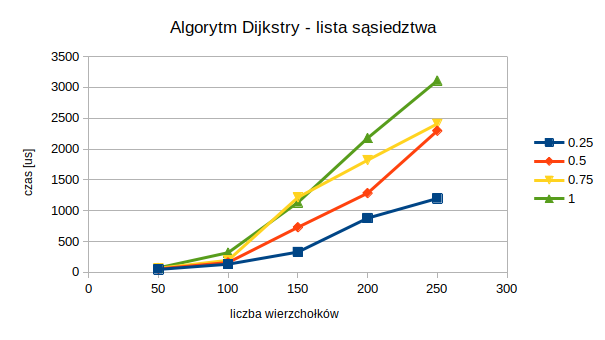
\includegraphics[width=13cm]{images/dijkstralista.png}
    \caption{ Algorytm Dijkstry dla listy sąsiedztwa}
\end{figure}

\paragraph{Macierz incydencji}

\begin{table}[H]
    \centering
    \begin{tabular}{|l|llll|}
        \hline
                                             & \multicolumn{4}{c|}{gęstość {[}\%{]}}                                                                        \\ \hline
        \multirow{2}{*}{liczba wierzchołków} & \multicolumn{1}{l|}{25}               & \multicolumn{1}{l|}{0.5}    & \multicolumn{1}{l|}{0.75}    & 1       \\ \cline{2-5}
                                             & \multicolumn{4}{c|}{[μs]}                                                                                    \\ \hline
        50                                   & \multicolumn{1}{l|}{299.5}            & \multicolumn{1}{l|}{571}    & \multicolumn{1}{l|}{799.8}   & 1042.2  \\ \hline
        100                                  & \multicolumn{1}{l|}{2033.5}           & \multicolumn{1}{l|}{5667.6} & \multicolumn{1}{l|}{11381.7} & 16495.8 \\ \hline
        150                                  & \multicolumn{1}{l|}{13420}            & \multicolumn{1}{l|}{48753}  & \multicolumn{1}{l|}{108020}  & 112149  \\ \hline
        200                                  & \multicolumn{1}{l|}{61269.1}          & \multicolumn{1}{l|}{134872} & \multicolumn{1}{l|}{192799}  & 260884  \\ \hline
        250                                  & \multicolumn{1}{l|}{130317}           & \multicolumn{1}{l|}{215626} & \multicolumn{1}{l|}{258153}  & 398347  \\ \hline
    \end{tabular}
    \caption{pomiary czasu wykonania algorytmu Dijkstry dla macierzy incydencji}
\end{table}

\begin{figure}[H]
    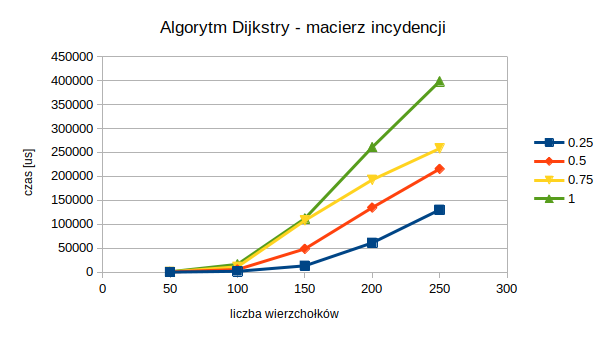
\includegraphics[width=13cm]{images/dijkstramacierz.png}
    \caption{ Algorytm Dijkstry dla listy sąsiedztwa}
\end{figure}

\subsubsection{Algorytm Bellmana-Forda}
\paragraph{Lista sąsiedztwa}
\begin{table}[H]
    \centering
    \begin{tabular}{|l|llll|}
        \hline
                                             & \multicolumn{4}{c|}{gęstość {[}\%{]}}                                                                         \\ \hline
        \multirow{2}{*}{liczba wierzchołków} & \multicolumn{1}{l|}{25}               & \multicolumn{1}{l|}{0.5}     & \multicolumn{1}{l|}{0.75}    & 1       \\ \cline{2-5}
                                             & \multicolumn{4}{c|}{[μs]}                                                                                     \\ \hline
        50                                   & \multicolumn{1}{l|}{250.6}            & \multicolumn{1}{l|}{396.1}   & \multicolumn{1}{l|}{568.8}   & 737     \\ \hline
        100                                  & \multicolumn{1}{l|}{1563.7}           & \multicolumn{1}{l|}{3120.1}  & \multicolumn{1}{l|}{5207.9}  & 7742.5  \\ \hline
        150                                  & \multicolumn{1}{l|}{6985.3}           & \multicolumn{1}{l|}{18057.3} & \multicolumn{1}{l|}{36367.8} & 39566.2 \\ \hline
        200                                  & \multicolumn{1}{l|}{23917.4}          & \multicolumn{1}{l|}{48260.1} & \multicolumn{1}{l|}{69151.2} & 104654  \\ \hline
        250                                  & \multicolumn{1}{l|}{47897.9}          & \multicolumn{1}{l|}{81855.6} & \multicolumn{1}{l|}{113067}  & 219050  \\ \hline
    \end{tabular}
    \caption{pomiary czasu wykonania algorytmu Bellmana-Forda dla listy sąsiedztwa}
\end{table}

\begin{figure}[H]
    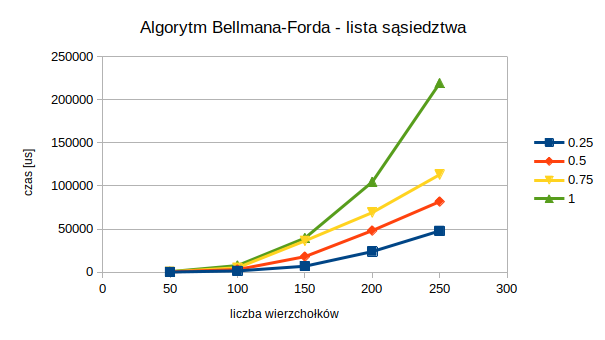
\includegraphics[width=13cm]{images/bellmanlista.png}
    \caption{ Algorytm Bellmana-Forda dla listy sąsiedztwa}
\end{figure}
\paragraph{Macierz incydencji}

\begin{table}[H]
    \begin{tabular}{|l|llll|}
        \hline
                                             & \multicolumn{4}{c|}{gęstość {[}\%{]}}                                                                            \\ \hline
        \multirow{2}{*}{liczba wierzchołków} & \multicolumn{1}{l|}{25}               & \multicolumn{1}{l|}{0.5}      & \multicolumn{1}{l|}{0.75}     & 1        \\ \cline{2-5}
                                             & \multicolumn{4}{c|}{[μs]}                                                                                        \\ \hline
        50                                   & \multicolumn{1}{l|}{13369.4}          & \multicolumn{1}{l|}{26014.6}  & \multicolumn{1}{l|}{38133.8}  & 52723.9  \\ \hline
        100                                  & \multicolumn{1}{l|}{187129}           & \multicolumn{1}{l|}{375414}   & \multicolumn{1}{l|}{593878}   & 961387   \\ \hline
        150                                  & \multicolumn{1}{l|}{1207240}          & \multicolumn{1}{l|}{3562990}  & \multicolumn{1}{l|}{5432010}  & 5714210  \\ \hline
        200                                  & \multicolumn{1}{l|}{4485500}          & \multicolumn{1}{l|}{10295800} & \multicolumn{1}{l|}{13878700} & 17832100 \\ \hline
        250                                  & \multicolumn{1}{l|}{11906300}         & \multicolumn{1}{l|}{19413200} & \multicolumn{1}{l|}{24039800} & 35827200 \\ \hline
    \end{tabular}
    \caption{pomiary czasu wykonania algorytmu Bellmana-Forda dla   macierzy incydencji}
\end{table}

\begin{figure}[H]
    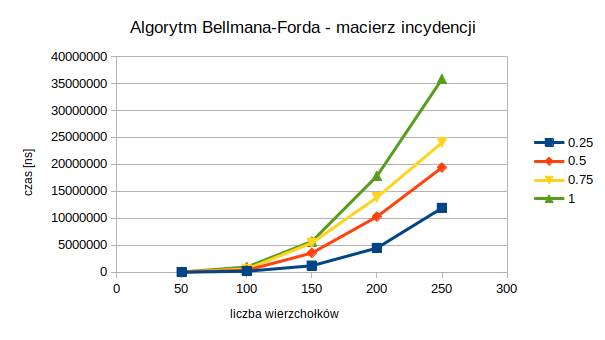
\includegraphics[width=13cm]{images/bellmanmacierz.png}
    \caption{ Algorytm Bellmana-Forda dla macierzy incydencji}
\end{figure}

\paragraph{Porównanie algorytmów}
\begin{figure}[H]
    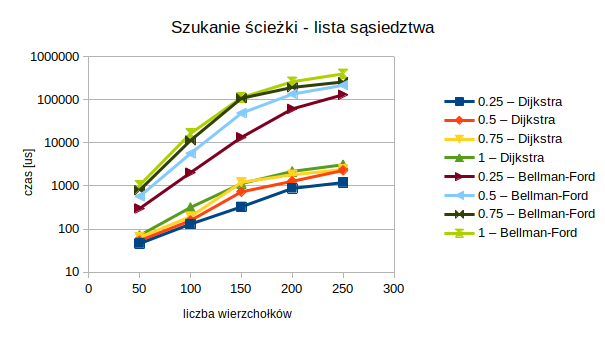
\includegraphics[width=13cm]{images/dijkstrabellmanlista.png}
    \caption{ Porównanie algorytmów Dijkstry i Bellmana-Forda dla listy sąsiedztwa}
\end{figure}

\begin{figure}[H]
    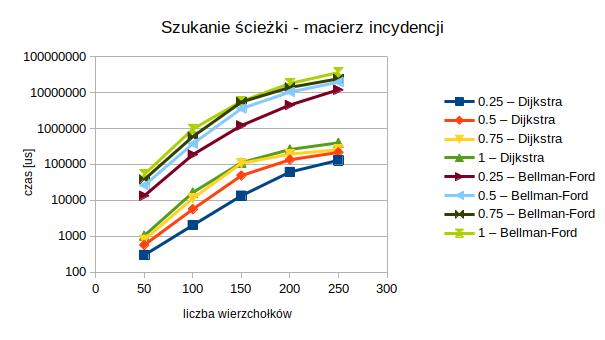
\includegraphics[width=13cm]{images/dijkstrabellmanmacierz.png}
    \caption{ Porównanie algorytmów Dijkstry i Bellmana-Forda dla macierzy incydencji}
\end{figure}

\begin{figure}[H]
    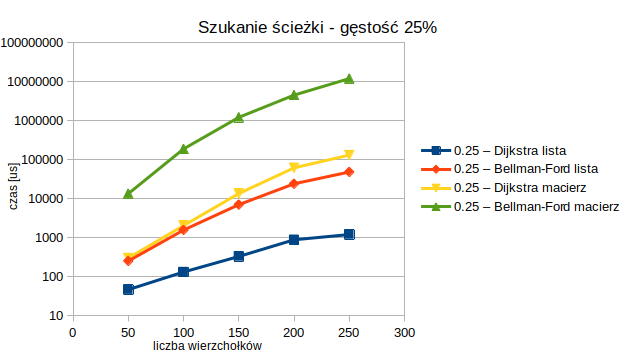
\includegraphics[width=13cm]{images/db25.png}
    \caption{ Porównanie algorytmów Dijkstry i Bellmana-Forda dla gęstości grafu 25\%}
\end{figure}

\begin{figure}[H]
    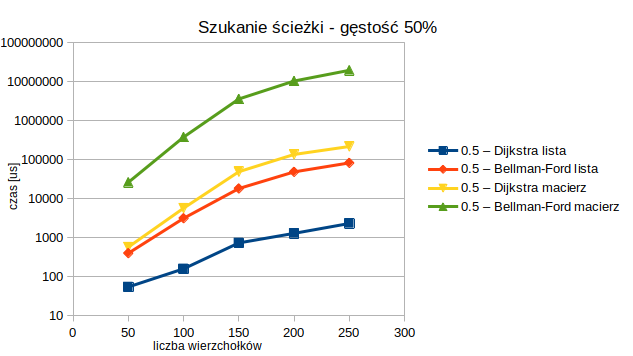
\includegraphics[width=13cm]{images/db50.png}
    \caption{ Porównanie algorytmów Dijkstry i Bellmana-Forda dla gęstości grafu 50\%}
\end{figure}

\begin{figure}[H]
    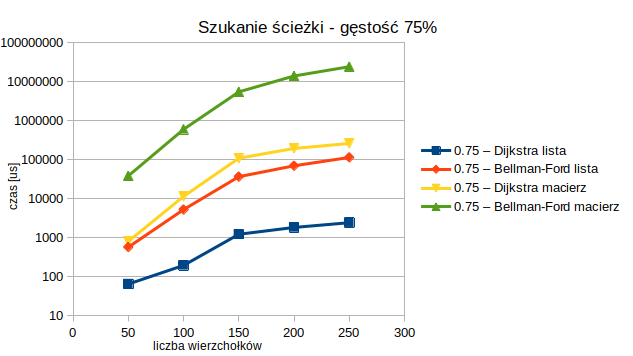
\includegraphics[width=13cm]{images/db75.png}
    \caption{ Porównanie algorytmów Dijkstry i Bellmana-Forda dla gęstości grafu 75\%}
\end{figure}

\begin{figure}[H]
    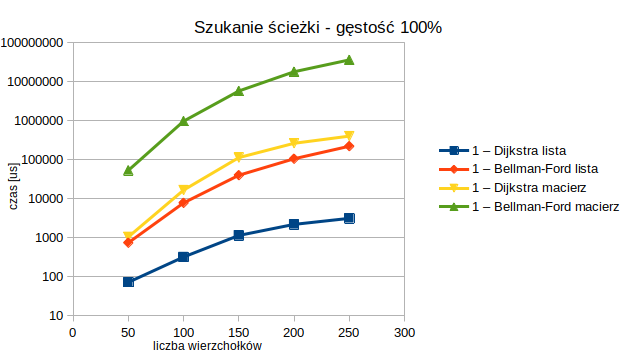
\includegraphics[width=13cm]{images/db100.png}
    \caption{ Porównanie algorytmów Dijkstry i Bellmana-Forda dla gęstości grafu 100\%}
\end{figure}

\subsection{Wyznaczanie minimalnego drzewa rozpinającego}
\subsubsection{Algorytm Prima}
\paragraph{Lista sąsiedztwa}
\begin{table}[H]
    \centering
    \begin{tabular}{|l|llll|}
        \hline
                                             & \multicolumn{4}{c|}{gęstość {[}\%{]}}                                                                      \\ \hline
        \multirow{2}{*}{liczba wierzchołków} & \multicolumn{1}{l|}{25}               & \multicolumn{1}{l|}{0.5}    & \multicolumn{1}{l|}{0.75}   & 1      \\ \cline{2-5}
                                             & \multicolumn{4}{c|}{[μs]}                                                                                  \\ \hline
        50                                   & \multicolumn{1}{l|}{98.8}             & \multicolumn{1}{l|}{190.5}  & \multicolumn{1}{l|}{179.4}  & 214.7  \\ \hline
        100                                  & \multicolumn{1}{l|}{653}              & \multicolumn{1}{l|}{988.2}  & \multicolumn{1}{l|}{1284.3} & 1542.2 \\ \hline
        150                                  & \multicolumn{1}{l|}{2080.3}           & \multicolumn{1}{l|}{2528}   & \multicolumn{1}{l|}{2435.1} & 2860.5 \\ \hline
        200                                  & \multicolumn{1}{l|}{3154.5}           & \multicolumn{1}{l|}{3574.2} & \multicolumn{1}{l|}{4469.9} & 7028.4 \\ \hline
        250                                  & \multicolumn{1}{l|}{3558.9}           & \multicolumn{1}{l|}{4014.8} & \multicolumn{1}{l|}{4771.8} & 6659   \\ \hline
    \end{tabular}
    \caption{pomiary czasu wykonania algorytmu Prima dla listy sąsiedztwa}
\end{table}
\begin{figure}[H]
    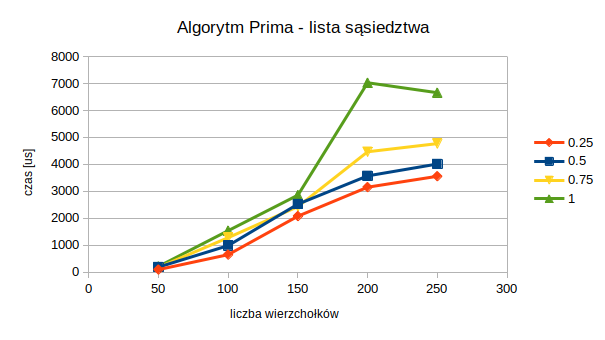
\includegraphics[width=13cm]{images/primlista.png}
    \caption{ Algorytm Prima dla listy sąsiedztwa}
\end{figure}

\paragraph{Macierz incydencji}
\begin{table}[H]
    \centering
    \begin{tabular}{|l|llll|}
        \hline
                                             & \multicolumn{4}{c|}{gęstość {[}\%{]}}                                                                           \\ \hline
        \multirow{2}{*}{liczba wierzchołków} & \multicolumn{1}{l|}{25}               & \multicolumn{1}{l|}{0.5}     & \multicolumn{1}{l|}{0.75}     & 1        \\ \cline{2-5}
                                             & \multicolumn{4}{c|}{[μs]}                                                                                       \\ \hline
        50                                   & \multicolumn{1}{l|}{4381.4}           & \multicolumn{1}{l|}{15213.3} & \multicolumn{1}{l|}{26397.5}  & 33037.7  \\ \hline
        100                                  & \multicolumn{1}{l|}{90108.1}          & \multicolumn{1}{l|}{333725}  & \multicolumn{1}{l|}{672840}   & 747975   \\ \hline
        150                                  & \multicolumn{1}{l|}{607973}           & \multicolumn{1}{l|}{1731790} & \multicolumn{1}{l|}{2523640}  & 2891450  \\ \hline
        200                                  & \multicolumn{1}{l|}{1585600}          & \multicolumn{1}{l|}{4863460} & \multicolumn{1}{l|}{7595420}  & 9919720  \\ \hline
        250                                  & \multicolumn{1}{l|}{3943070}          & \multicolumn{1}{l|}{8135320} & \multicolumn{1}{l|}{13663200} & 15632200 \\ \hline
    \end{tabular}
    \caption{pomiary czasu dla wykonania algorytmu Prima dla macierzy incydencji}
    \label{tab:my-table}
\end{table}
\begin{figure}[H]
    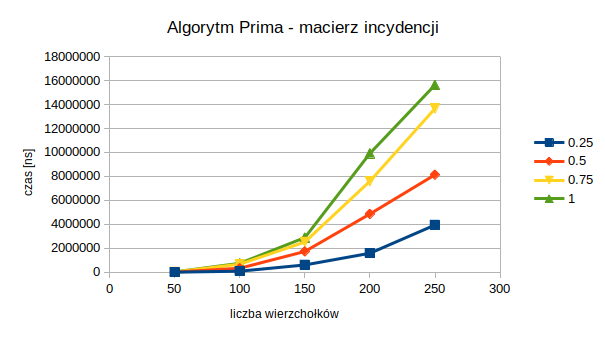
\includegraphics[width=13cm]{images/primmacierz.png}
    \caption{ Algorytm Prima dla    macierzy incydencji}
\end{figure}

\subsubsection{Algorytm Kruskala}

\paragraph{Lista sąsiedztwa}
\begin{table}[H]
    \centering
    \begin{tabular}{|l|llll|}
        \hline
                                             & \multicolumn{4}{c|}{gęstość {[}\%{]}}                                                                           \\ \hline
        \multirow{2}{*}{liczba wierzchołków} & \multicolumn{1}{l|}{25}               & \multicolumn{1}{l|}{0.5}     & \multicolumn{1}{l|}{0.75}     & 1        \\ \cline{2-5}
                                             & \multicolumn{4}{c|}{[μs]}                                                                                       \\ \hline
        50                                   & \multicolumn{1}{l|}{4565.2}           & \multicolumn{1}{l|}{14198.3} & \multicolumn{1}{l|}{25529.2}  & 32219.9  \\ \hline
        100                                  & \multicolumn{1}{l|}{87859.4}          & \multicolumn{1}{l|}{328322}  & \multicolumn{1}{l|}{617719}   & 675654   \\ \hline
        150                                  & \multicolumn{1}{l|}{565339}           & \multicolumn{1}{l|}{1696130} & \multicolumn{1}{l|}{2362380}  & 2939720  \\ \hline
        200                                  & \multicolumn{1}{l|}{1528330}          & \multicolumn{1}{l|}{4639590} & \multicolumn{1}{l|}{7264690}  & 9622900  \\ \hline
        250                                  & \multicolumn{1}{l|}{3733480}          & \multicolumn{1}{l|}{7927100} & \multicolumn{1}{l|}{13720300} & 15649900 \\ \hline
    \end{tabular}
    \caption{pomiary czasu dla wykonania algorytmu Kruskala dla listy sąsiedztwa}
    \label{tab:my-table}
\end{table}
\begin{figure}[H]
    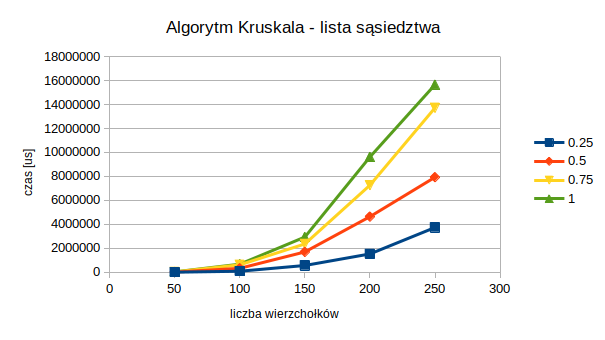
\includegraphics[width=13cm]{images/kruskallista.png}
    \caption{ Algorytm Prima dla    macierzy incydencji}
\end{figure}
\paragraph{Macierz incydencji}

\begin{table}[H]
    \centering
    \begin{tabular}{|l|llll|}
        \hline
                                             & \multicolumn{4}{c|}{gęstość {[}\%{]}}                                                                           \\ \hline
        \multirow{2}{*}{liczba wierzchołków} & \multicolumn{1}{l|}{25}               & \multicolumn{1}{l|}{0.5}     & \multicolumn{1}{l|}{0.75}     & 1        \\ \cline{2-5}
                                             & \multicolumn{4}{c|}{[μs]}                                                                                       \\ \hline
        50                                   & \multicolumn{1}{l|}{4644}             & \multicolumn{1}{l|}{15416.8} & \multicolumn{1}{l|}{27019.4}  & 32967    \\ \hline
        100                                  & \multicolumn{1}{l|}{91866}            & \multicolumn{1}{l|}{323097}  & \multicolumn{1}{l|}{658338}   & 723943   \\ \hline
        150                                  & \multicolumn{1}{l|}{611020}           & \multicolumn{1}{l|}{1753970} & \multicolumn{1}{l|}{2451020}  & 2892360  \\ \hline
        200                                  & \multicolumn{1}{l|}{1617660}          & \multicolumn{1}{l|}{4913760} & \multicolumn{1}{l|}{7556850}  & 9982490  \\ \hline
        250                                  & \multicolumn{1}{l|}{3949320}          & \multicolumn{1}{l|}{8132030} & \multicolumn{1}{l|}{14187800} & 15877500 \\ \hline
    \end{tabular}
    \caption{pomiary czasu dla wykonania algorytmu kruskala dla macierzy incydencji}
    \label{tab:my-table}
\end{table}
\begin{figure}[H]
    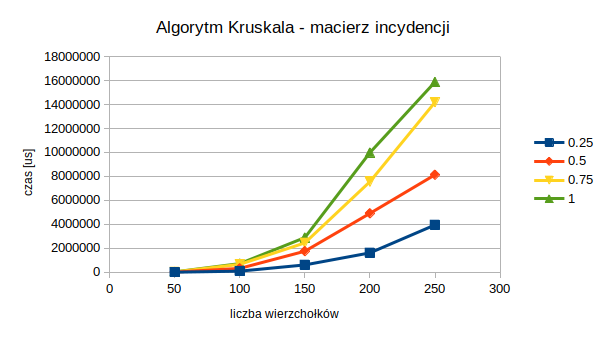
\includegraphics[width=13cm]{images/kruskalmacierz.png}
    \caption{ Algorytm Prima dla    macierzy incydencji}
\end{figure}

\paragraph{Porównanie algorytmów}

\begin{figure}[H]
    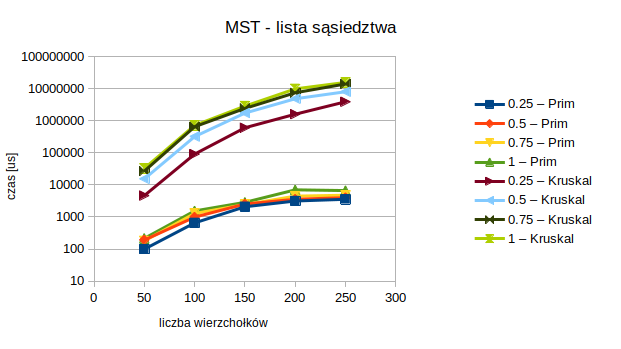
\includegraphics[width=13cm]{images/mstlista.png}
    \caption{ Porównanie algorytmów Prima i Kruskala dla listy sąsiedztwa}
\end{figure}

\begin{figure}[H]
    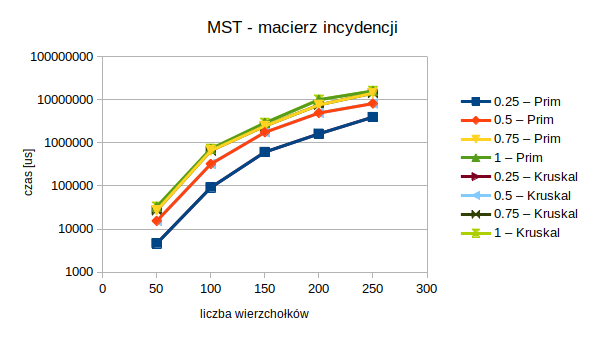
\includegraphics[width=13cm]{images/mstmacierz.png}
    \caption{ Porównanie algorytmów Prima i Kruskala dla macierzy incydencji}
\end{figure}

\begin{figure}[H]
    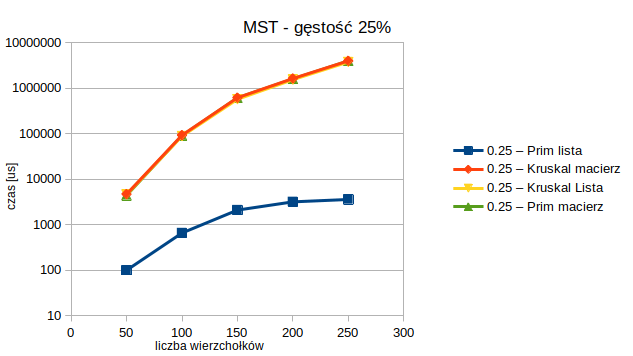
\includegraphics[width=13cm]{images/mst25.png}
    \caption{ Porównanie algorytmów Prima i Kruskala dla gęstości grafu 25\%}
\end{figure}

\begin{figure}[H]
    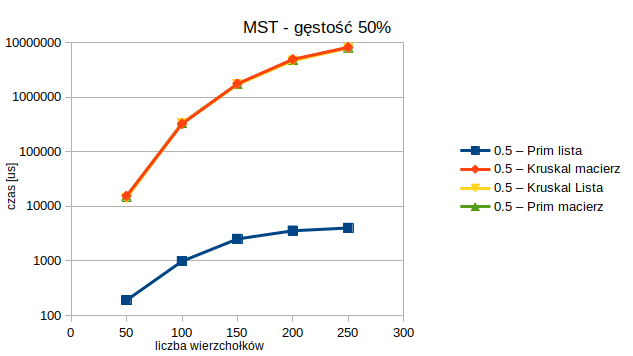
\includegraphics[width=13cm]{images/mst50.png}
    \caption{ Porównanie algorytmów Prima i Kruskala dla gęstości grafu 50\%}
\end{figure}


\begin{figure}[H]
    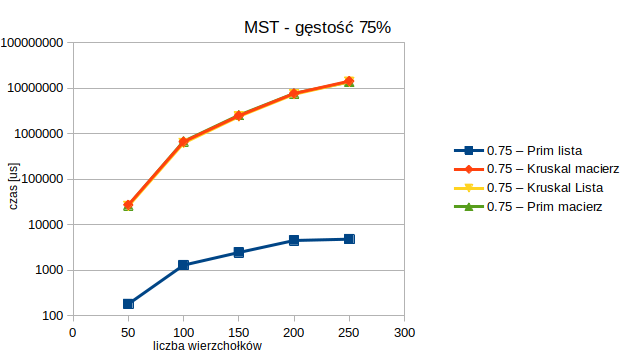
\includegraphics[width=13cm]{images/mst75.png}
    \caption{ Porównanie algorytmów Prima i Kruskala dla gęstości grafu 75\%}
\end{figure}


\begin{figure}[H]
    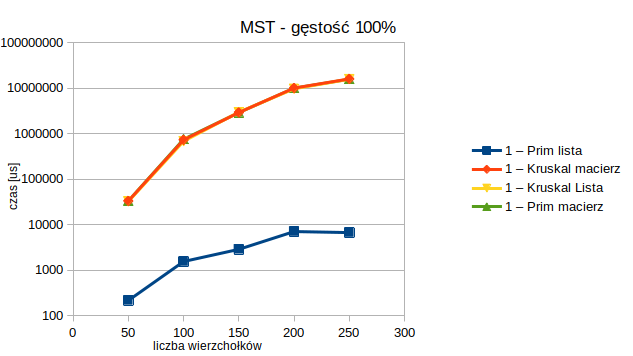
\includegraphics[width=13cm]{images/mst100.png}
    \caption{ Porównanie algorytmów Prima i Kruskala dla gęstości grafu 100\%}
\end{figure}


\section{Wnioski}

Dla algorytmów wyszukiwania najkrótszej ścieżki, algorytm Dijkstry jest znacznie szybszy od algorytmu Bellmana-Forda.
Z kolei dla algorytmów wyszukiwania minimalnego drzewa rozpinającego, algorytm Prima jest znacznie szybszy od algorytmu Kruskala.
Rozróżniając algorytmy po reprezentacji grafu, algorytmy dla listy sąsiedztwa są znacznie szybsze od algorytmów dla macierzy incydencji.
Dzieję się tak, ponieważ dla macierzy incydencji algorytm musi najpierw znaleźć odpowiednie krawędzie, przeszukując praktycznie całą macierz.
Z kolei dla listy sąsiedztwa, algorytm musi jedynie przejść przez listę sąsiedztwa danego wierzchołka.

Złoności obliczeniowe algorytmów różnią się od tych teoretycznych, ponieważ w programie wykorzystywane są struktury danych, które nie są optymalne (przykładem możę być tutaj struktura implementująca tablicę dynamiczną, gdzie zajmuje ona możliwe najmniej miejsca). Oraz przy implementacji algorytmów nie zawsze wykorzystywane są optymalne rozwiązania.
Takie jak korzystanie z kolejki piorytetowej, czy kopca minimanlnego, które są optymalne dla poszczególnych algorytmów.

\begin{thebibliography}{9}
    \bibitem{texbook}
    Thomas H. Cormen, Charles E. Leiserson, Ron Rivest, Clifford Stein (2022) \emph{Introduction to algorithms 4th edition}, MIT Press and McGraw-Hill.
    \bibitem{texbook}
    Prezentacje dr inż. Jarosława Mierzwy
\end{thebibliography}
\end{document}